\documentclass[journal]{IEEEtran}

\usepackage[T1]{fontenc}
\usepackage[utf8]{inputenc}
\usepackage{amsmath,amssymb,amsfonts}
\usepackage{graphicx}
\usepackage{booktabs}
\usepackage{array}
\usepackage{url}
\usepackage{xcolor}
\usepackage[hidelinks]{hyperref}
\usepackage{orcidlink}
\usepackage{balance}

\graphicspath{{../figures/}}

\renewcommand{\topfraction}{0.92}
\renewcommand{\bottomfraction}{0.75}
\renewcommand{\textfraction}{0.08}
\renewcommand{\floatpagefraction}{0.80}

% IEEEtran hard-codes an em-dash after the abstract and index-terms names; the CAOS
% content standard (ADR-0067) excludes em-dashes, so the separator is a full stop.
\makeatletter
\def\abstract{\normalfont
    \if@twocolumn
      \@IEEEabskeysecsize\bfseries\textit{\abstractname}.\ \relax
    \else
      \bgroup\par\addvspace{0.5\baselineskip}\centering\vspace{-1.78ex}\@IEEEabskeysecsize\textbf{\abstractname}\par\addvspace{0.5\baselineskip}\egroup\quotation\@IEEEabskeysecsize
    \fi\@IEEEgobbleleadPARNLSP}
\def\IEEEkeywords{\normalfont
    \if@twocolumn
      \@IEEEabskeysecsize\bfseries\textit{\IEEEkeywordsname}.\ \relax
    \else
      \bgroup\par\addvspace{0.5\baselineskip}\centering\@IEEEabskeysecsize\textbf{\IEEEkeywordsname}\par\addvspace{0.5\baselineskip}\egroup\quotation\@IEEEabskeysecsize
    \fi\@IEEEgobbleleadPARNLSP}
\makeatother

% Numbers quoted in the text are read from the committed artifacts by figures/make_figs.py.
% generated by figures/make_figs.py from the committed artifacts; do not edit
\newcommand{\BackKwCov}{0.9}
\newcommand{\BackKwLpd}{$-$5.85}
\newcommand{\BackKwMape}{25.94}
\newcommand{\BackKwRmse}{78.52}
\newcommand{\BackKwWidth}{209.79}
\newcommand{\BackTphCov}{0.8}
\newcommand{\BackTphLpd}{$-$6.90}
\newcommand{\BackTphMape}{12.09}
\newcommand{\BackTphRmse}{176.67}
\newcommand{\BackTphWidth}{473.76}
\newcommand{\BlinKwCov}{0.8}
\newcommand{\BlinKwLpd}{$-$5.34}
\newcommand{\BlinKwMape}{12.78}
\newcommand{\BlinKwRmse}{44.56}
\newcommand{\BlinKwWidth}{119.60}
\newcommand{\BlinTphCov}{0.8}
\newcommand{\BlinTphLpd}{$-$6.71}
\newcommand{\BlinTphMape}{13.67}
\newcommand{\BlinTphRmse}{177.75}
\newcommand{\BlinTphWidth}{478.76}
\newcommand{\FreeKwCov}{0.8}
\newcommand{\FreeKwLpd}{$-$5.40}
\newcommand{\FreeKwMape}{14.03}
\newcommand{\FreeKwRmse}{48.68}
\newcommand{\FreeKwWidth}{129.82}
\newcommand{\FreeTphCov}{0.8}
\newcommand{\FreeTphLpd}{$-$6.65}
\newcommand{\FreeTphMape}{12.18}
\newcommand{\FreeTphRmse}{174.42}
\newcommand{\FreeTphWidth}{468.51}
\newcommand{\accMax}{0.204}
\newcommand{\accMin}{0.171}
\newcommand{\bondKwMax}{237}
\newcommand{\bondKwMin}{196}
\newcommand{\burn}{1000}
\newcommand{\calKwMax}{419}
\newcommand{\calKwMin}{365}
\newcommand{\cbKwCov}{0.9}
\newcommand{\cbKwLpd}{$-$5.35}
\newcommand{\cbKwMape}{14.31}
\newcommand{\cbKwRmse}{44.68}
\newcommand{\cbKwWidth}{117.74}
\newcommand{\cbTphCov}{0.8}
\newcommand{\cbTphLpd}{$-$6.68}
\newcommand{\cbTphMape}{12.00}
\newcommand{\cbTphRmse}{168.57}
\newcommand{\cbTphWidth}{439.12}
\newcommand{\constKwMape}{24.48}
\newcommand{\constTphMape}{18.29}
\newcommand{\covHi}{0.9}
\newcommand{\covLo}{0.7}
\newcommand{\cssMax}{55}
\newcommand{\cssMin}{38}
\newcommand{\dKwConstContr}{0.910}
\newcommand{\dKwConstMean}{$-$12.57}
\newcommand{\dKwConstPriorSd}{36.00}
\newcommand{\dKwConstSd}{32.77}
\newcommand{\dKwCssContr}{0.381}
\newcommand{\dKwCssMean}{$-$57.07}
\newcommand{\dKwCssPriorSd}{36.00}
\newcommand{\dKwCssSd}{13.70}
\newcommand{\dKwFContr}{0.362}
\newcommand{\dKwFMean}{$-$5.16}
\newcommand{\dKwFPriorSd}{36.00}
\newcommand{\dKwFSd}{13.03}
\newcommand{\dKwPerMm}{$-$9.6}
\newcommand{\dTphConstContr}{0.878}
\newcommand{\dTphConstMean}{53.36}
\newcommand{\dTphConstPriorSd}{140.00}
\newcommand{\dTphConstSd}{122.88}
\newcommand{\dTphCssContr}{0.350}
\newcommand{\dTphCssMean}{100.84}
\newcommand{\dTphCssPriorSd}{140.00}
\newcommand{\dTphCssSd}{49.00}
\newcommand{\dTphFContr}{0.340}
\newcommand{\dTphFMean}{56.57}
\newcommand{\dTphFPriorSd}{140.00}
\newcommand{\dTphFSd}{47.63}
\newcommand{\dTphPerMm}{17.0}
\newcommand{\draws}{20}
\newcommand{\fEightyMax}{140}
\newcommand{\fEightyMin}{47}
\newcommand{\gainBackTph}{0.09}
\newcommand{\gainBlinKw}{$-$1.53}
\newcommand{\kOneScaleContr}{0.965}
\newcommand{\kOneScaleMean}{1.07}
\newcommand{\kOneScalePriorSd}{0.15}
\newcommand{\kOneScaleSd}{0.15}
\newcommand{\kThreeContr}{0.992}
\newcommand{\kThreeMean}{2.23}
\newcommand{\kThreePriorSd}{0.49}
\newcommand{\kThreeSd}{0.49}
\newcommand{\kTwoScaleContr}{1.026}
\newcommand{\kTwoScaleMean}{1.05}
\newcommand{\kTwoScalePriorSd}{0.15}
\newcommand{\kTwoScaleSd}{0.16}
\newcommand{\kwMMax}{355}
\newcommand{\kwMMin}{187}
\newcommand{\marginPts}{3.0}
\newcommand{\morrellMape}{38.08}
\newcommand{\morrellNoloadMape}{15.21}
\newcommand{\nIdent}{7}
\newcommand{\nNone}{5}
\newcommand{\nParams}{16}
\newcommand{\nPart}{4}
\newcommand{\nPosteriors}{11}
\newcommand{\nSamples}{12000}
\newcommand{\nSurveys}{10}
\newcommand{\noiseMedKw}{15}
\newcommand{\noiseMedTph}{60}
\newcommand{\pnContr}{0.795}
\newcommand{\pnMean}{86.35}
\newcommand{\pnPriorSd}{47.85}
\newcommand{\pnSd}{38.04}
\newcommand{\postSteps}{6000}
\newcommand{\qRefContr}{0.454}
\newcommand{\qRefMean}{646.35}
\newcommand{\qRefNominal}{647}
\newcommand{\qRefPriorSd}{167.01}
\newcommand{\qRefSd}{75.74}
\newcommand{\rEngCss}{0.79}
\newcommand{\rMeasCss}{$-$0.82}
\newcommand{\ratioMax}{125.0}
\newcommand{\ratioMin}{70.7}
\newcommand{\samplerVersion}{3.1.6}
\newcommand{\sdCss}{5.9}
\newcommand{\seed}{42}
\newcommand{\sha}{483d24c5ddd35b41f2be05628fe9f09fd22562c5ab59cda69e036b9bb0ce605a}
\newcommand{\shaDoc}{2ad1ae736c7c8a6559be448ea6fa67b732d051e17ea7d8be7487863f7e0fb96c}
\newcommand{\shuffleTphMape}{25.04}
\newcommand{\sigKwContr}{0.332}
\newcommand{\sigKwMean}{38.81}
\newcommand{\sigKwPriorSd}{32.42}
\newcommand{\sigKwSd}{10.75}
\newcommand{\sigTphContr}{0.301}
\newcommand{\sigTphMean}{145.23}
\newcommand{\sigTphPriorSd}{129.67}
\newcommand{\sigTphSd}{39.04}
\newcommand{\steps}{7000}
\newcommand{\tShiftContr}{0.990}
\newcommand{\tShiftMean}{$-$0.11}
\newcommand{\tShiftPriorSd}{3.99}
\newcommand{\tShiftSd}{3.95}
\newcommand{\tauFactor}{50}
\newcommand{\tauKw}{36}
\newcommand{\tauMax}{84.8}
\newcommand{\tauMin}{48.0}
\newcommand{\tauTph}{140}
\newcommand{\thin}{10}
\newcommand{\tphMMax}{1639}
\newcommand{\tphMMin}{813}
\newcommand{\walkers}{20}
\newcommand{\wiContr}{0.854}
\newcommand{\wiMean}{8.39}
\newcommand{\wiPriorSd}{1.52}
\newcommand{\wiSd}{1.29}
\newcommand{\widthRedKw}{43.9}
\newcommand{\widthRedTph}{7.3}
\newcommand{\zetaContr}{0.733}
\newcommand{\zetaMean}{1.14}
\newcommand{\zetaPriorSd}{0.30}
\newcommand{\zetaSd}{0.22}


% Page-1 header block (conventions/manuscript-header-standard.md). The four document
% macros are set by the publishing tool when the version DOI is reserved.
\newcommand{\doctype}{Preprint}
\newcommand{\docversion}{v0.01}
\newcommand{\docdate}{31 October 2026}
\newcommand{\versiondoi}{10.5281/zenodo.23843810}
\newcommand{\conceptdoi}{10.5281/zenodo.23843809}
\newcommand{\docrepo}{github.com/fsantibanezleal/CAOS\_ChancaDEM}
\newcommand{\headerblock}{%
\begin{center}
\fbox{\parbox{0.94\textwidth}{\small\raggedright
\textbf{\doctype} \quad$\cdot$\quad \docversion, \docdate \quad$\cdot$\quad Licence CC BY 4.0\\[2pt]
CAOS open-research programme \quad$\cdot$\quad CAOS\_ChancaDEM, crusher comminution studio\\[2pt]
Version DOI \href{https://doi.org/\versiondoi}{\texttt{\versiondoi}} \quad$\cdot$\quad
concept DOI (always latest) \href{https://doi.org/\conceptdoi}{\texttt{\conceptdoi}}\\[2pt]
Not peer reviewed. Source code, data and computational records: \href{https://\docrepo}{\texttt{\docrepo}}
}}
\end{center}
\vspace{4pt}}

\newcommand{\pct}{\,\%}

\begin{document}

\title{What Ten Industrial Surveys Identify in a Cone-Crusher Population Balance Model: Bayesian Calibration with Structural Discrepancy}

\author{Felipe~Santib\'a\~nez-Leal~\orcidlink{0000-0002-0150-3246}%
\thanks{F. Santib\'a\~nez-Leal is with the CAOS open-research programme, Santiago, Chile
(e-mail: fsantibanez@gmail.com; ORCID 0000-0002-0150-3246).}%
\thanks{Interactive studio and reproducible pipeline (MIT) at
\url{https://github.com/fsantibanezleal/CAOS_ChancaDEM}.}}

\markboth{{}\doctype\ \docversion, 2026}%
{Santib\'a\~nez-Leal: What ten industrial surveys identify in a cone-crusher population balance model}

\IEEEaftertitletext{\vspace{-0.6\baselineskip}\headerblock\vspace{0.2\baselineskip}}

\maketitle

\begin{abstract}
A cone-crusher model that predicts throughput, power and product size rests on a handful of fitted scalars, and a point
fit to a few industrial surveys does not say which of them the surveys determine. We calibrate the eight fitted scalars
of a Whiten classification-breakage population balance engine of a Metso HP500 cone crusher (capacity, Bond work
index, power form, classification and breakage constants) as a Bayesian posterior against the ten surveys of Rocha et
al., with a linear structural discrepancy on the closed-side setting and the feed size in the form of Kennedy and
O'Hagan. The posterior is sampled with the differential-evolution moves of ter Braak, after the affine-invariant
stretch move failed an autocorrelation-time criterion on the same posterior. Strict leave-one-survey-out validation
refits every quantity without the held-out survey. Held out, the posterior predictive mean has a mean absolute
percentage error of \cbTphMape\pct{} on throughput and \cbKwMape\pct{} on power, which is within the noise of a
setting-only line (\BlinTphMape\pct{} and \BlinKwMape\pct{}) and no gain over it on power. The 80\pct{} bands cover
\cbTphCov{} and \cbKwCov{} of the surveys, and on power the band is \widthRedKw\pct{} narrower than the residual band of
the refit backbone at the same coverage; against the setting-only line (width \BlinKwWidth~kW, coverage \BlinKwCov{}) and the
free-form fit (\FreeKwWidth~kW, \FreeKwCov{}) its width of \cbKwWidth~kW is about the same, with a higher coverage, so the band gain is against the backbone and not
against the simple line. Of the \nParams{} parameters, \nIdent{} are identified by the surveys; the
classification and breakage scalars of the population balance stay at their prior. With ten surveys and no measured
product size, the data calibrate how the two outputs depend on the setting, and they cannot calibrate the population
balance.
\end{abstract}

\begin{IEEEkeywords}
Cone crusher, population balance, Bayesian calibration, model discrepancy, identifiability, leave-one-out validation,
differential-evolution MCMC, comminution.
\end{IEEEkeywords}

\section{Introduction}

\IEEEPARstart{T}{he} electricity of a copper concentrator goes especially to crushing and grinding, and in Chile in 2024 the
concentrators took 55.7\,\% of the electricity of copper mining~\cite{cochilco}. A cone crusher is modelled in the
tradition of Whiten~\cite{whiten}: a classification function decides which particles are broken, a breakage function
distributes the progeny, and a mass balance gives the product. The classification constants, the breakage law, the
capacity and the power form of such an engine are fitted to survey data, and the fitted values are then used as if they
were known.

Industrial surveys of a crusher are few and expensive. Rocha et al.~\cite{rocha} report ten surveys of an HP500 secondary
cone crusher on itabirite iron ore with five numbers each: the closed-side setting (CSS), the feed size
$f_{80}$, the throughput and the motor power, and a product size distribution that appears only as a figure. A point fit
to ten rows of two measured outputs raises two questions that the point fit does not answer. Which of the fitted scalars
do the surveys determine, and which does the fit leave where it started? And how well calibrated is the prediction of an
unseen survey?

We answer both with a Bayesian calibration of the engine with an explicit structural discrepancy. The engine is run as
its own simulator (a few milliseconds per evaluation), the eight fitted scalars get weakly informative priors centred
on the values of Rocha et al., and a linear discrepancy on the setting and the feed size is added to each measured
output in the form of Kennedy and O'Hagan~\cite{ko}. The result is a posterior per scalar, a predictive distribution per
held-out survey and a table of prior against posterior. Our contributions are:
\begin{enumerate}
\item a Bayesian calibration with discrepancy of a cone-crusher population balance engine, with the discrepancy
integrated out exactly so that the sampler explores ten dimensions only;
\item a sampler configuration chosen by a measured criterion: the differential-evolution moves meet an
autocorrelation-time criterion that the stretch move does not meet on the same posterior;
\item a strict leave-one-survey-out evaluation over the ten surveys, against a setting-only line, a refit backbone with
a residual band and a free-form linear fit, with calibration (coverage and width) scored beside accuracy;
\item the identifiability table: which scalars the surveys determine, which they determine partly and which stay at
their prior, and the structural discrepancy that the power output requires.
\end{enumerate}
The calibrated prediction is not more accurate than a line in the closed-side setting. The result is the
identifiability finding and a calibrated predictive band, not a gain in point accuracy.

\section{Related Work}

\subsection{Calibration with discrepancy}

Kennedy and O'Hagan~\cite{ko} calibrate the parameters of a computer model against field data by writing the data as
the simulator at the true parameters plus a model discrepancy, itself a Gaussian process, plus measurement error.
Higdon et al.~\cite{higdon} extend the construction to a simulator that cannot be run at every
parameter value, with Gaussian process models of the unknown functions, and Bayarri et al.~\cite{bayarri} give a
six-step Bayesian framework for validating a computer model against reality. Brynjarsd\'ottir and
O'Hagan~\cite{brynj} show that an analysis that ignores the model discrepancy can give biased and over-confident
parameter estimates and predictions, and that the confounding of the discrepancy with the calibration parameters is
resolved only with meaningful priors. We use the low-order form: the discrepancy is linear in the standardized setting and feed
size, with a Gaussian prior on its three coefficients per output. The engine is cheap, so no emulator is used.

\subsection{Samplers}

The affine-invariant ensemble sampler of Goodman and Weare~\cite{gw}, implemented in \texttt{emcee}~\cite{emcee}, moves a
walker along the line to another walker (the stretch move). ter Braak~\cite{tb06} proposed differential-evolution
Markov chain Monte Carlo, a multiple-chain sampler whose jumps are built from differences between chains, and ter Braak and
Vrugt~\cite{tbv08} added a snooker updater so that fewer than twice the dimension of chains suffice. Both families are gradient free, which
matters here because the engine solves a linear system per evaluation and is written in plain Python.

\subsection{Crusher models and their calibration}

Rocha et al.~\cite{rocha} fitted a model of the HP500 on the same ten surveys and published the fitted expressions for
the classification constants, the breakage parameter, the capacity and the power form; they are the nominal values of
our priors. Lindqvist and Li~\cite{lindq} present a cone-crusher model with a coupled energy and breakage dependency.
Morrell~\cite{morrell} gives a size-specific energy for crushing circuits that we use as a comparator for power. The
engine itself combines the Whiten balance~\cite{whiten}, the JKMRC breakage and classification relations~\cite{napier},
Evertsson's capacity model~\cite{evertsson} and Bond's law~\cite{bond}. Literature searches in Crossref and on the open
web for a Bayesian calibration with discrepancy of a crusher or mill population balance model returned general
methodology and no application to a cone crusher evaluated on held-out surveys; the search is not exhaustive, because
Scopus and Web of Science were not searched.

\section{Method}

\subsection{Data}

The data are the ten surveys of the Metso HP500 secondary cone crusher at an itabirite iron-ore operation (Table~\ref{tab:surveys}
of Appendix~\ref{app:data}): the closed-side setting spans \cssMin\ to \cssMax~mm, the feed $f_{80}$ \fEightyMin\ to
\fEightyMax~mm, the throughput \tphMMin\ to \tphMMax~t/h and the motor power \kwMMin\ to \kwMMax~kW. Throughput and power
are the two targets. The product $P_{80}$ is not measured (the product size distributions of the source are figures
only), so it is never a target.

\subsection{The engine}

For a survey with setting $c$ and feed size $f_{80}$ the engine evaluates a classification-breakage balance on a
size grid. The classification function is zero below $K_1$, one above $K_2$ and
\begin{equation}
C(d)=1-\left(\frac{K_2-d}{K_2-K_1}\right)^{K_3}\quad (K_1<d<K_2),
\end{equation}
with $K_1=s_{K_1}(0.23\,c+0.30\,f_{80})$ and $K_2=\max\{s_{K_2}(12.0+0.55\,c+0.40\,f_{80}),\,1.05\,K_1\}$ in mm, the
coefficients being those of Rocha et al.~\cite{rocha} and $s_{K_1}$, $s_{K_2}$ multipliers. The breakage function
follows from the $t_{10}$ relation $t_{10}\,(\%)=64+\Delta t_{10}-0.12\,c-0.23\,f_{80}$, capped at 44, through the
appearance function of Austin. The product mass fractions are $\mathbf p=(\mathbf I-\mathbf C)(\mathbf I-\mathbf B\mathbf C)^{-1}\mathbf f$ for a
feed $\mathbf f$ reconstructed from the measured $f_{80}$ with a Rosin--Rammler distribution of uniformity $0.9$. The
throughput depends on the setting and one scalar,
\begin{equation}
Q=Q_{\mathrm{ref}}\;\sigma(c),
\end{equation}
where $\sigma(c)$ is the capacity factor of the machine, linear in the setting, at the fixed throw of 34~mm and
speed of 360~rpm. The Bond power and the calibrated power are
\begin{align}
P_d &= 10\,W_i\left(\frac{1}{\sqrt{P_{80}}}-\frac{1}{\sqrt{f_{80}}}\right) Q,\\
P_c &= \zeta\,P_d+P_n,
\end{align}
with the sizes in micrometres, $W_i$ the Bond work index of the ore blend, and $\zeta$ and $P_n$ the slope and the no-load
power of the current-based form of Rocha et al.~\cite{rocha}. The eight scalars $\boldsymbol\theta=(Q_{\mathrm{ref}},W_i,\zeta,P_n,s_{K_1},s_{K_2},K_3,\Delta t_{10})$ are the
quantities calibrated. Two facts of the structure matter for what the surveys can identify. Throughput depends on
$Q_{\mathrm{ref}}$ alone: the other seven scalars never enter it. Power depends on all eight, the four of the population
balance ($s_{K_1}$, $s_{K_2}$, $K_3$, $\Delta t_{10}$) only through the product size $P_{80}$ in the Bond term, and
$W_i$ and $\zeta$ only through their product.

\subsection{Priors}

Each scalar has a truncated normal prior around its nominal value, on the logarithmic scale for the positive scalars
(Table~\ref{tab:priors}). The nominal values are those of Rocha et al.~\cite{rocha} (Tables 4 and 5) and, for $W_i$, the
blend of the compact and supercompact itabirite bands (7.2 and 10.6~kWh/t, Table 1 of the same work). The widths are
weakly informative choices that bracket the spans quoted there; we found no published range of these fitted scalars for
this ore, so the widths are ours. The noise scale of each output has $\ln\sigma_t\sim N(\ln m_t,1)$ with medians
$m_{\mathrm{tph}}=\noiseMedTph$~t/h and $m_{\mathrm{kW}}=\noiseMedKw$~kW, about 5\,\% of the typical level.

\begin{table}[!t]
\caption{Priors of the eight engine scalars. The sampled scale is the natural logarithm for the positive scalars.}
\label{tab:priors}
\centering\footnotesize
\resizebox{\columnwidth}{!}{\begin{tabular}{@{}llrrl@{}}
\toprule
Scalar & Unit & Nominal & Prior (sampled scale) & Range \\
\midrule
$Q_{\mathrm{ref}}$ & t/h & 647.00 & $\ln x \sim N(6.47,\,0.25^2)$ & 300.00 to 1400.0 \\
$W_i$ & kWh/t & 9.00 & $\ln x \sim N(2.20,\,0.17^2)$ & 5.00 to 14.0 \\
$\zeta$ & -- & 1.30 & $\ln x \sim N(0.26,\,0.23^2)$ & 0.50 to 2.5 \\
$P_n$ & kW & 110.00 & $N(110.0,\,50.0^2)$ & 0.0 to 300.0 \\
$s_{K_1}$ & -- & 1.00 & $\ln x \sim N(0.00,\,0.15^2)$ & 0.50 to 2.0 \\
$s_{K_2}$ & -- & 1.00 & $\ln x \sim N(0.00,\,0.15^2)$ & 0.50 to 2.0 \\
$K_3$ & -- & 2.30 & $N(2.3,\,0.5^2)$ & 1.0 to 4.0 \\
$\Delta t_{10}$ & points of $t_{10}$ & 0.00 & $N(0.0,\,4.0^2)$ & $-$15.0 to 15.0 \\
\bottomrule
\end{tabular}
}
\end{table}

\subsection{Discrepancy and likelihood}

For survey $i$ and output $t\in\{\mathrm{tph},\mathrm{kW}\}$,
\begin{equation}
y_{t,i}=f_t(\boldsymbol\theta;c_i,f_{80,i})+\delta_t(\mathbf z_i)+\varepsilon_{t,i},\quad \varepsilon_{t,i}\sim N(0,\sigma_t^2),
\end{equation}
\begin{equation}
\delta_t(\mathbf z)=d_{t,0}+d_{t,1}z_{c}+d_{t,2}z_{f_{80}},\quad d_{t,j}\sim N(0,\tau_t^2),
\end{equation}
where $\mathbf z$ is the pair (setting, feed size) standardized with the mean and standard deviation of the training
surveys, and $\tau_{\mathrm{tph}}=\tauTph$~t/h and $\tau_{\mathrm{kW}}=\tauKw$~kW (about 12\,\% of the typical level). Given
$\boldsymbol\theta$ and $\sigma_t$ the model is linear and Gaussian in $\mathbf d_t$, so the discrepancy is integrated out
exactly: with $\mathbf Z$ the $n\times3$ matrix of rows $(1,z_c,z_{f_{80}})$ of the training surveys,
\begin{equation}
\mathbf y_t\sim N\!\left(\mathbf f_t(\boldsymbol\theta),\ \sigma_t^2\mathbf I+\tau_t^2\mathbf Z\mathbf Z^{\top}\right).
\label{eq:marginal}
\end{equation}
The two outputs are treated as independent given $\boldsymbol\theta$, and the likelihood is the product of the two
densities in~\eqref{eq:marginal}. The sampler explores the eight scalars and the two noise scales (ten dimensions). For
each retained sample the discrepancy coefficients are drawn from their exact Gaussian conditional given the residual, and
the posterior predictive of a held-out survey is the engine at that survey plus $\mathbf x_h^\top\mathbf d_t$ plus
noise, with $\mathbf x_h$ the standardized regressors of the survey. The interval of 80\,\% is the 10th to the 90th
percentile of \draws{} predictive draws per retained sample.

\subsection{Sampler and convergence}

The sampler is \texttt{emcee} \samplerVersion~\cite{emcee} with the differential-evolution move and the snooker move
of ter Braak~\cite{tb06} and ter Braak and Vrugt~\cite{tbv08}, in proportions 0.8 and 0.2, with \walkers{} walkers, \steps{}
steps, the first \burn{} discarded and every \thin{}th kept, which retains \nSamples{} samples per posterior, and a fixed
seed (\seed). The walkers start in a small ball around the prior centre (5\,\% of the prior standard deviation).

The affine-invariant stretch move of Goodman and Weare~\cite{gw} was the first choice. On the same posterior it did
not converge by the criterion below: the integrated autocorrelation time stayed above 100 steps and grew with the chain
length, along the parameters that the surveys do not identify, so that no fold met the criterion at \steps{} steps. The
differential-evolution moves reach an autocorrelation time of about 50 steps on the same posterior within the same
number of steps. The held-out scores hardly depend on the move: the power MAPE is 14.29\pct{} with the stretch move
and \cbKwMape\pct{} with the differential-evolution moves, and the throughput MAPE is \cbTphMape\pct{} with both.

A posterior counts as converged when the post-burn chain is at least \tauFactor{} integrated autocorrelation times long, with
the autocorrelation time of \texttt{emcee} (the largest over the ten dimensions). A posterior that fails the criterion is
reported as not converged.

\section{Experiments}

\subsection{Strict leave-one-survey-out}

For each of the ten surveys, a posterior is computed from the other nine surveys alone: the engine scalars, the noise
scales, the discrepancy and the standardization of the regressors are all refit inside the fold, and the held-out survey
enters only the prediction. One more posterior is computed from all ten surveys for the identifiability table. That
makes \nPosteriors{} posteriors.

\subsection{Comparators}

The three comparators are refit inside every fold on the nine training surveys.
\begin{itemize}
\item The \emph{setting-only line} is an ordinary least-squares line of the output on the closed-side setting. It has no
physics.
\item The \emph{refit backbone} is the engine at the nominal scalars with the capacity base $Q_{\mathrm{ref}}$ refit for
throughput, and the slope and intercept of the form $P_c=\zeta P_d+P_n$ refit for power, both by least squares. Its
80\,\% band is the \emph{residual band}: the prediction plus or minus 1.2816 times the standard deviation of the held-out
residuals of the other nine surveys, so that a survey never enters the width of its own band.
\item The \emph{free-form linear fit} is an ordinary least-squares fit of the output on the setting and the feed size.
\end{itemize}
The bands of the setting-only line and of the free-form fit are built in the same way as the residual band. For power,
Morrell's size-specific energy~\cite{morrell} is held out as well, with its work index refit per fold, with and without a
no-load term; it reaches \morrellMape\pct{} and \morrellNoloadMape\pct{}, and its fitted work index is negative in every
fold with the no-load term, so that variant is a descriptive line and not an estimate of the work index.

\subsection{Scores}

Per output: the mean absolute percentage error (MAPE) of the predictive mean; the root mean squared error (RMSE, in t/h
or kW); the mean log predictive density of the held-out measurement (a log density per t/h or per kW, higher is better;
for CrusherBayes the log of the mean of the Gaussian densities over the posterior draws, for the comparators a Gaussian
with the residual-band standard deviation); the coverage of the 80\,\% interval, which is the fraction of surveys whose
measurement lies inside; and the mean width of that interval. With $n=10$ one survey moves a coverage by 0.1, and a
difference of about \marginPts{} points of MAPE is within the noise.

\subsection{Rule for dropping the method, stated before the run}

Before the posteriors were computed we stated when the method would be dropped as a predictor: (a) its power MAPE is not
below that of the setting-only line by at least \marginPts{} points and its throughput MAPE is not below that of the refit
backbone by at least \marginPts{} points, and (b) on either output its coverage lies outside \covLo{} to \covHi{} or its mean band is wider
than the residual band. Both conditions must hold. Whatever the outcome, the identifiability table is reported.

\section{Results}

\subsection{Held-out accuracy and calibration}

Table~\ref{tab:accuracy} gives the scores. On throughput the posterior predictive mean has a MAPE of
\cbTphMape\pct{}, against \BackTphMape\pct{} for the refit backbone, \FreeTphMape\pct{} for the free-form fit and
\BlinTphMape\pct{} for the setting-only line; a constant mean gives \constTphMape\pct{}. The differences of the first
four are below the noise level of ten surveys. On power the posterior predictive mean has a MAPE of \cbKwMape\pct{},
against \BackKwMape\pct{} for the refit backbone, \FreeKwMape\pct{} for the free-form fit and \BlinKwMape\pct{} for the
setting-only line, \BlinKwMape\pct{} being the lowest; a constant mean gives \constKwMape\pct{}. CrusherBayes
therefore removes most of the error of the refit backbone on power, and it does not beat the line in the setting: its gain
over the line is \gainBlinKw{} points, which is within the noise. This is a measured negative result for accuracy.

The calibration is better than that of the backbone and comparable to that of the simple models. The 80\,\% interval of CrusherBayes covers \cbTphCov{} of the surveys for throughput and
\cbKwCov{} for power, both inside \covLo{} to \covHi{}. Its mean width is \cbTphWidth~t/h on throughput, \widthRedTph\pct{}
narrower than the residual band of the refit backbone (\BackTphWidth~t/h) at the same coverage, and \cbKwWidth~kW on
power, \widthRedKw\pct{} narrower than the residual band (\BackKwWidth~kW) at the same coverage of \cbKwCov{}. On power
the comparison with the simple models is different: the setting-only line has a mean width of \BlinKwWidth~kW and covers \BlinKwCov{} of the
surveys, and the free-form fit has \FreeKwWidth~kW and \FreeKwCov{}, against \cbKwWidth~kW and \cbKwCov{} for CrusherBayes. Its width is
about that of the setting-only line, whose coverage is lower, so the gain in band width on power is against the backbone and not against the simple line.
On throughput its width is smaller than that of the setting-only line (\BlinTphWidth~t/h) and of the free-form fit (\FreeTphWidth~t/h), all with coverage \cbTphCov{}.
Figure~\ref{fig:band} shows the bands against the measured values survey by survey.

\begin{table}[!t]
\caption{Held-out scores over the ten surveys (strict leave-one-survey-out). Coverage and width are those of the 80\,\% interval.}
\label{tab:accuracy}
\centering\footnotesize
\resizebox{\columnwidth}{!}{\begin{tabular}{@{}llrrrrr@{}}
\toprule
Target & Method & MAPE (\%) & RMSE & Mean log density & Coverage & Width \\
\midrule
\multicolumn{7}{@{}l}{\textit{Throughput (t/h)}} \\
& CrusherBayes & 12.00 & 168.57 & $-$6.678 & 0.8 & 439.1 \\
& Setting-only line & 13.67 & 177.75 & $-$6.709 & 0.8 & 478.8 \\
& Refit backbone with residual band & 12.09 & 176.67 & $-$6.896 & 0.8 & 473.8 \\
& Free-form linear fit & 12.18 & 174.42 & $-$6.647 & 0.8 & 468.5 \\
\midrule
\multicolumn{7}{@{}l}{\textit{Power (kW)}} \\
& CrusherBayes & 14.31 & 44.68 & $-$5.346 & 0.9 & 117.7 \\
& Setting-only line & 12.78 & 44.56 & $-$5.341 & 0.8 & 119.6 \\
& Refit backbone with residual band & 25.94 & 78.52 & $-$5.847 & 0.9 & 209.8 \\
& Free-form linear fit & 14.03 & 48.68 & $-$5.399 & 0.8 & 129.8 \\
\bottomrule
\end{tabular}
}
\end{table}

\begin{figure*}[!t]
\centering
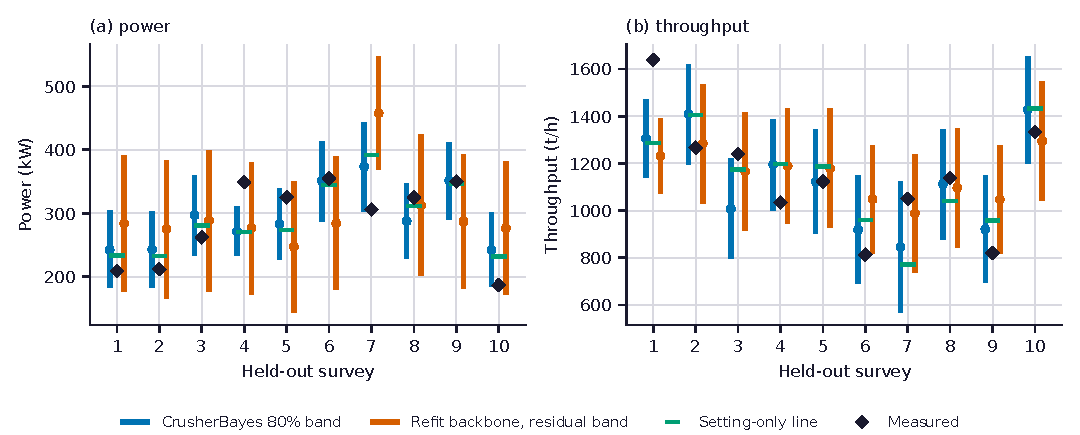
\includegraphics[width=0.9\textwidth]{fig-band.pdf}
\caption{Held-out 80\,\% predictive interval against the measured value, per survey, for (a) power and (b) throughput.
The blue interval is the posterior predictive of CrusherBayes and the orange interval the residual band of the refit
backbone; the green dash is the setting-only line and the black diamond the measurement. Every interval is computed
without the survey it is drawn for.}
\label{fig:band}
\end{figure*}

\subsection{Outcome of the dropping rule}

Table~\ref{tab:rule} applies the rule stated before the run. Condition (a) holds: the gain in power MAPE over the setting-only
line is \gainBlinKw{} points and the gain in throughput MAPE over the refit backbone is \gainBackTph{} points, both below
\marginPts{}. Condition (b) fails: the coverages \cbTphCov{} and \cbKwCov{} are inside the interval \covLo{} to \covHi{}, and the
bands are narrower than the residual band on both outputs. As both conditions are needed to drop the method, the rule does
not drop it. The rule, as written, therefore retains a method that calibrates its band and does not improve the point
prediction; it does not assert a gain in accuracy.

\begin{table}[!t]
\caption{The terms of the rule for dropping the method as a predictor, evaluated on the held-out scores. The reference is the setting-only line for power and the refit backbone for throughput.}
\label{tab:rule}
\centering\footnotesize
\begin{tabular}{@{}lrr@{}}
\toprule
Term & Throughput & Power \\
\midrule
MAPE of CrusherBayes (\%) & 12.00 & 14.31 \\
MAPE of the reference (\%) & 12.09 & 12.78 \\
Gain over the reference (points) & 0.09 & $-$1.53 \\
Gain of at least 3 points & no & no \\
Coverage & 0.8 & 0.9 \\
Coverage outside 0.7 to 0.9 & no & no \\
Mean width (t/h, kW) & 439.1 & 117.7 \\
Mean width of the residual band & 473.8 & 209.8 \\
Band wider than the residual band & no & no \\
\bottomrule
\end{tabular}

\end{table}

\subsection{What the surveys identify}

Table~\ref{tab:identifiability} compares the prior with the posterior of every parameter, fitted to all ten surveys. The
ratio is the posterior standard deviation over the prior standard deviation; a ratio far below one means that the surveys
determine the parameter, a ratio near one that it stays at its prior. We read a ratio up to 0.5 as identified, up to
0.9 as partly identified and above 0.9 as at its prior; a ratio slightly above one (\kTwoScaleContr{} for
$s_{K_2}$) is read as no contraction. Figure~\ref{fig:posterior} shows the prior and a normal summary of the posterior for
each parameter, and Fig.~\ref{fig:contraction} the ratios.

\begin{table*}[!t]
\caption{Prior against posterior of the \nParams{} parameters, fitted to all ten surveys. The ratio is the posterior standard deviation over the prior standard deviation (natural scale).}
\label{tab:identifiability}
\centering\footnotesize
\begin{tabular}{@{}llrrrrrrl@{}}
\toprule
Parameter & Unit & Nominal (prior median) & Prior mean & Prior SD & Posterior mean & Posterior SD & Ratio & Reading \\
\midrule
$Q_{\mathrm{ref}}$ & t/h & 647.00 & 667.13 & 167.01 & 646.35 & 75.74 & 0.454 & identified \\
$W_i$ & kWh/t & 9.00 & 9.11 & 1.52 & 8.39 & 1.29 & 0.854 & partly identified \\
$\zeta$ & -- & 1.30 & 1.33 & 0.30 & 1.14 & 0.22 & 0.733 & partly identified \\
$P_n$ & kW & 110.00 & 111.83 & 47.85 & 86.35 & 38.04 & 0.795 & partly identified \\
$s_{K_1}$ & -- & 1.00 & 1.01 & 0.15 & 1.07 & 0.15 & 0.965 & not contracted \\
$s_{K_2}$ & -- & 1.00 & 1.01 & 0.15 & 1.05 & 0.16 & 1.026 & not contracted \\
$K_3$ & -- & 2.30 & 2.31 & 0.49 & 2.23 & 0.49 & 0.992 & not contracted \\
$\Delta t_{10}$ & points & 0.00 & 0.00 & 3.99 & $-$0.11 & 3.95 & 0.990 & not contracted \\
\midrule
$\sigma_{\mathrm{tph}}$ & t/h & 60.00 & 98.92 & 129.67 & 145.23 & 39.04 & 0.301 & identified \\
$\sigma_{\mathrm{kW}}$ & kW & 15.00 & 24.73 & 32.42 & 38.81 & 10.75 & 0.332 & identified \\
\midrule
$d_{\mathrm{tph},0}$ & t/h & 0.00 & 0.00 & 140.00 & 53.36 & 122.88 & 0.878 & partly identified \\
$d_{\mathrm{tph},1}$ (setting) & t/h & 0.00 & 0.00 & 140.00 & 100.84 & 49.00 & 0.350 & identified \\
$d_{\mathrm{tph},2}$ ($f_{80}$) & t/h & 0.00 & 0.00 & 140.00 & 56.57 & 47.63 & 0.340 & identified \\
\midrule
$d_{\mathrm{kW},0}$ & kW & 0.00 & 0.00 & 36.00 & $-$12.57 & 32.77 & 0.910 & not contracted \\
$d_{\mathrm{kW},1}$ (setting) & kW & 0.00 & 0.00 & 36.00 & $-$57.07 & 13.70 & 0.381 & identified \\
$d_{\mathrm{kW},2}$ ($f_{80}$) & kW & 0.00 & 0.00 & 36.00 & $-$5.16 & 13.03 & 0.362 & identified \\
\bottomrule
\end{tabular}

\end{table*}

\begin{figure*}[!t]
\centering
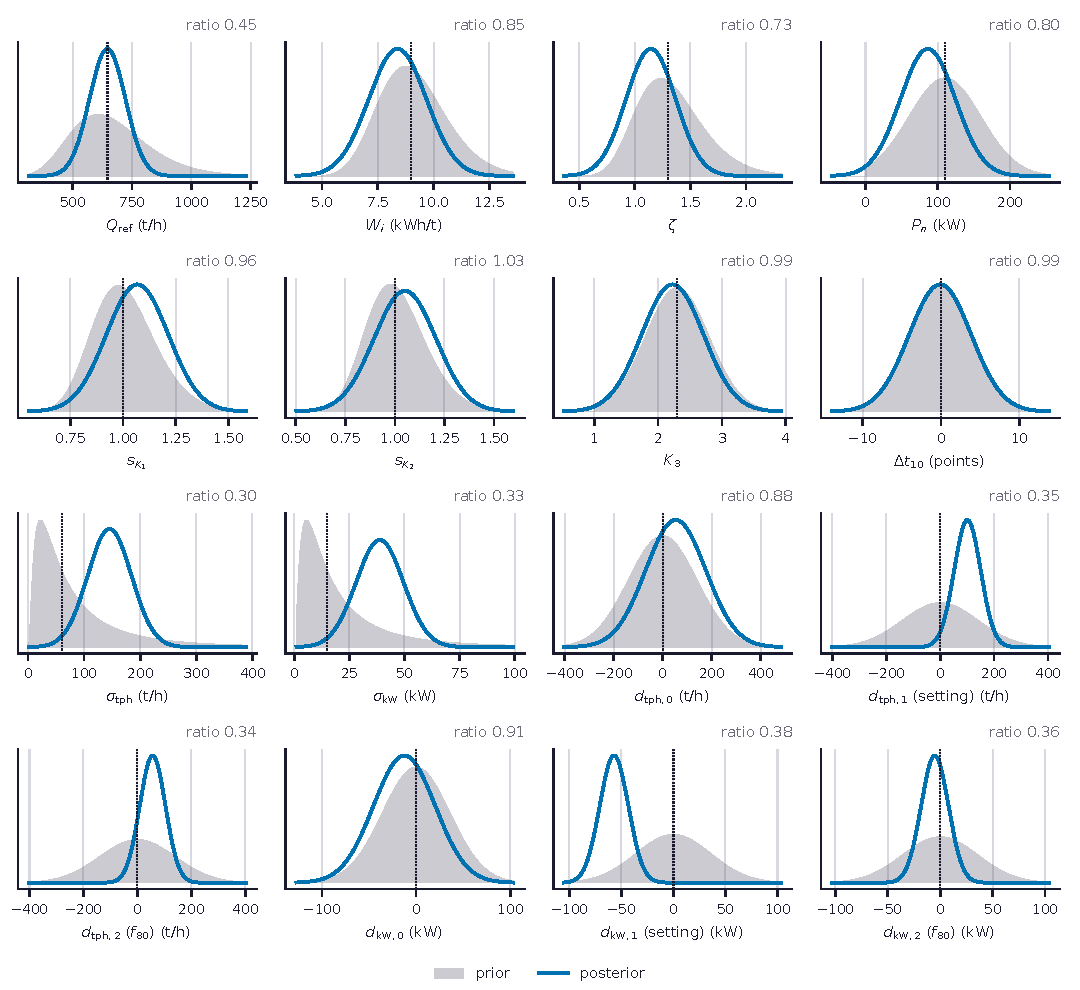
\includegraphics[width=0.8\textwidth]{fig-posterior.pdf}
\caption{Prior (grey area) against posterior (blue line) of each parameter, fitted to all ten surveys. The posterior is drawn
as a normal density with its mean and standard deviation, the two summaries of the fit; the dotted line is the nominal
value. The ratio is the posterior over the prior standard deviation.}
\label{fig:posterior}
\end{figure*}

\begin{figure}[!t]
\centering
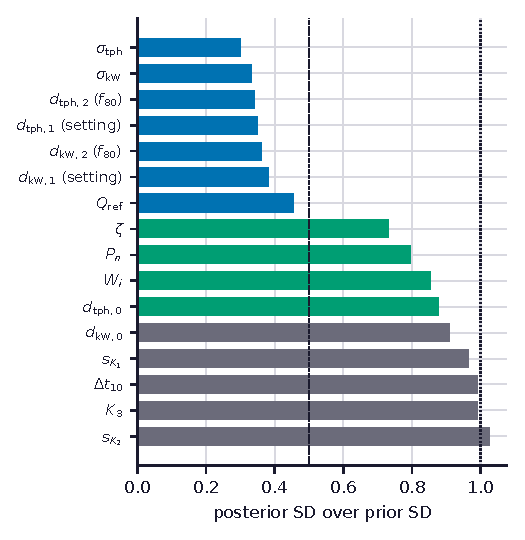
\includegraphics[width=0.78\columnwidth]{fig-contraction.pdf}
\caption{Posterior over prior standard deviation of each parameter: identified (blue, up to 0.5), partly identified
(green, up to 0.9) and at the prior (grey). The dashed line marks 0.5 and the dotted line 1.}
\label{fig:contraction}
\end{figure}

Of the \nParams{} parameters, \nIdent{} are identified, \nPart{} are partly identified and \nNone{} stay at their prior. The
identified ones are the capacity base $Q_{\mathrm{ref}}$ (ratio \qRefContr{}), the two noise scales (\sigTphContr{} for
throughput, \sigKwContr{} for power) and the four discrepancy slopes on the setting and the feed size
(\dTphCssContr{} to \dKwCssContr{}). Partly identified are $\zeta$ (\zetaContr{}), $P_n$ (\pnContr{}), $W_i$
(\wiContr{}) and the constant of the throughput discrepancy (\dTphConstContr{}). Four of the eight engine scalars stay at
their prior: the multipliers $s_{K_1}$ (\kOneScaleContr{}) and $s_{K_2}$ (\kTwoScaleContr{}), the exponent $K_3$
(\kThreeContr{}) and the breakage shift $\Delta t_{10}$ (\tShiftContr{}), and so does the constant of the power
discrepancy (\dKwConstContr{}). The posterior mean of $Q_{\mathrm{ref}}$ is \qRefMean~t/h against a nominal \qRefNominal~t/h:
the surveys narrow the capacity base and leave its centre where it was.

\subsection{The discrepancy}

The discrepancy slope on the setting is large for both outputs. For power it is \dKwCssMean{} $\pm$ \dKwCssSd~kW per
standard deviation of the setting (about \dKwPerMm~kW/mm, with \sdCss~mm the standard deviation of the setting over the
ten surveys), and for throughput \dTphCssMean{} $\pm$ \dTphCssSd~t/h per standard deviation (about \dTphPerMm~t/h per mm).
The measured power falls as the setting widens (correlation \rMeasCss{}), whereas the calibrated engine power rises with
it (correlation \rEngCss{}, from \calKwMin\ to \calKwMax~kW over the ten surveys); the negative discrepancy slope of power has the opposite sign to the setting dependence of the engine, and
compensates it.

\subsection{Convergence}

All \nPosteriors{} posteriors meet the criterion (Table~\ref{tab:convergence} of Appendix~\ref{app:convergence}): the largest autocorrelation time is
between \tauMin{} and \tauMax{} steps and the \postSteps{} post-burn steps are \ratioMin{} to \ratioMax{} times it. The acceptance
fraction is between \accMin{} and \accMax{}.

\section{Discussion}

\paragraph{Why the point accuracy does not improve}
Throughput of the engine is $Q_{\mathrm{ref}}\sigma(c)$ with $\sigma$ linear in the setting, and the discrepancy adds a
term linear in the setting and the feed size. Measured power correlates with the setting at
\rMeasCss{}, and the engine's own power moves the other way. Once the discrepancy has absorbed that setting dependence, the
posterior predictive is close in form to a line in the setting and the feed size, which the setting-only line and the free-form fit
already are; this agrees with the ties in Table~\ref{tab:accuracy}, but we did not test it directly.

\paragraph{Why the population balance is not identified}
The two measured outputs carry the product size only through the Bond term of power, and power follows the setting and
the throughput, not the product size. The four scalars that set the product size ($s_{K_1}$, $s_{K_2}$, $K_3$,
$\Delta t_{10}$) therefore remain at their prior, and the engine's product size, which is not measured in the ten surveys,
is not validated by them. Measured product size distributions per survey would constrain these scalars directly. We did
not test that, because the distributions of the source are figures only.

\paragraph{Confounding of calibration and discrepancy}
Brynjarsd\'ottir and O'Hagan~\cite{brynj} show that the discrepancy is confounded with the calibration parameters.
Two instances appear here. The capacity base and the constant of the throughput discrepancy both set the level of
throughput, and only the first contracts strongly (\qRefContr{} against \dTphConstContr{}). And since $W_i$ and $\zeta$
multiply, power fixes their product and not each of them, which is why both are only partly identified. The posterior of
the individual scalars should not be read as an estimate of a physical value of the ore.

\paragraph{What the band is worth}
The band of the setting-only line, built from the spread of its held-out residuals, is as wide as the CrusherBayes band on power
(\BlinKwWidth{} against \cbKwWidth~kW), with a coverage of \BlinKwCov{} against \cbKwCov{}. The advantage of CrusherBayes
over the line is that its band comes from a generative model of the survey (engine, discrepancy and noise), so the
band carries the uncertainty of the scalars; whether it stays calibrated at a setting outside the surveyed range was not tested. The advantage over the refit backbone is plain in the data: the same coverage with a band \widthRedKw\pct{} narrower on power. Against the setting-only line the power width is about the same (\cbKwWidth{} against \BlinKwWidth~kW) and the coverage is higher (\cbKwCov{} against \BlinKwCov{}), a difference of one survey out of ten; the band gain is not against the simple line.

\section{Limitations}

\begin{itemize}
\item Ten surveys of one machine, one ore and one operation, with two measured outputs and two regressors. Coverage is coarse:
one survey moves it by 0.1, and the coverages of \cbTphCov{} and \cbKwCov{} do not distinguish a calibrated band from a
slightly miscalibrated one.
\item The widths of the priors and the discrepancy standard deviations $\tau_t$ are our choices; no sensitivity analysis of
the held-out scores or of the ratios to those choices was made, and the confounding of discrepancy and parameters is resolved only by meaningful priors~\cite{brynj}.
\item The discrepancy is linear in two standardized regressors with a fixed prior scale, not a Gaussian process with
estimated hyperparameters; the two outputs are independent given the scalars.
\item The throw and the speed are fixed at the machine's nominal values, and the feed gradation is reconstructed from
the measured $f_{80}$ with a Rosin--Rammler distribution of fixed uniformity, so neither the throw, the speed nor the feed
shape is calibrated.
\item The convergence criterion uses the autocorrelation time of a single ensemble with one seed, and we did not
run independent ensembles with other seeds. The comparison with the stretch move is a measurement on the same posterior,
reported from the preliminary runs, and was not repeated for this paper.
\item The rule for dropping the method is lenient: it drops a method only when it fails on accuracy and on calibration at
once, so it retains a method that does not improve accuracy.
\item The comparison with other crusher models is limited to the comparators of the Experiments section; the discrete-element
simulation of a crusher is not covered, and the search of the literature was not exhaustive.
\end{itemize}

\section{Conclusions}

Ten HP500 surveys, two measured outputs and a linear discrepancy identify the capacity base, the two noise scales and the
dependence of both outputs on the setting and the feed size. They determine the work index and the power form only as a
product, and they leave the classification and breakage scalars of the population balance at their prior. Strict
leave-one-survey-out validation shows a throughput MAPE of \cbTphMape\pct{} and a power MAPE of \cbKwMape\pct{} for the
posterior predictive mean, no better than a line in the closed-side setting (\BlinTphMape\pct{} and \BlinKwMape\pct{}), with
80\,\% bands that are \widthRedKw\pct{} narrower on power than the residual band of the refit backbone at the same
coverage; against the setting-only line the power band has about the same width (\cbKwWidth{} against \BlinKwWidth~kW) and a coverage of \cbKwCov{} against \BlinKwCov{}. The finding is negative for accuracy and positive for calibration and for identifiability: to calibrate the
population balance itself, the surveys need to measure the product size.

\appendices

\section{Reproducibility}\label{app:repro}

The artifacts of the paper are in the repository \path{github.com/fsantibanezleal/CAOS_ChancaDEM}. The posteriors are
sampled offline by the pipeline step of the data bake (\texttt{python} \path{data-pipeline/run.py} \texttt{hp500}), which writes
\path{data/derived/hp500/crusherbayes.json}; the engine, the priors, the likelihood, the sampler and the scores are in
\path{data-pipeline/pipeline/hp500/crusherbayes.py}. Every figure, table and number of this paper is regenerated from the committed
artifacts \texttt{crusherbayes.json}, \texttt{loo.json}, \texttt{backbone.json} and \path{data/examples/hp500-surveys.csv} by
\texttt{python} \path{manuscripts/crusherbayes/figures/make_figs.py}, which also writes the number-to-key table
\path{manuscripts/crusherbayes/data/claims.json}. The sampler is \texttt{emcee} \samplerVersion{} with seed \seed{}. The document carries the SHA-256 of its inputs,
\begin{center}\texttt{\tiny\sha}\end{center}
and the SHA-256 of the file read for this paper is
\begin{center}\texttt{\tiny\shaDoc}\end{center}

\section{Survey data}\label{app:data}

\begin{table}[!h]
\caption{The ten HP500 surveys (Rocha et al.~\cite{rocha}, Table A1, CC BY 4.0): closed-side setting, feed $f_{80}$, throughput and motor power.}
\label{tab:surveys}
\centering\footnotesize
\begin{tabular}{@{}rrrrr@{}}
\toprule
Survey & Setting (mm) & $f_{80}$ (mm) & Throughput (t/h) & Power (kW) \\
\midrule
1 & 54 & 88 & 1639 & 209 \\
2 & 54 & 84 & 1267 & 212 \\
3 & 48 & 47 & 1240 & 262 \\
4 & 48 & 88 & 1034 & 349 \\
5 & 48 & 62 & 1124 & 325 \\
6 & 40 & 79 & 813 & 355 \\
7 & 38 & 140 & 1050 & 306 \\
8 & 44 & 123 & 1138 & 325 \\
9 & 40 & 81 & 820 & 350 \\
10 & 55 & 81 & 1334 & 187 \\
\bottomrule
\end{tabular}

\end{table}

\section{Convergence per posterior}\label{app:convergence}

\begin{table}[!h]
\caption{Convergence of the \nPosteriors{} posteriors: the largest integrated autocorrelation time $\tau_{\max}$ over the ten dimensions, the
post-burn chain length in units of $\tau_{\max}$ (the criterion is \tauFactor{}), the mean acceptance fraction and the retained samples.}
\label{tab:convergence}
\centering\footnotesize
\resizebox{\columnwidth}{!}{\begin{tabular}{@{}lrrrr@{}}
\toprule
Posterior & $\tau_{\max}$ (steps) & Post-burn steps / $\tau_{\max}$ & Acceptance & Retained samples \\
\midrule
without survey 1 & 52.6 & 114.1 & 0.204 & 12000 \\
without survey 2 & 52.7 & 113.8 & 0.201 & 12000 \\
without survey 3 & 54.7 & 109.7 & 0.203 & 12000 \\
without survey 4 & 84.8 & 70.7 & 0.171 & 12000 \\
without survey 5 & 52.7 & 113.9 & 0.203 & 12000 \\
without survey 6 & 48.0 & 125.0 & 0.204 & 12000 \\
without survey 7 & 55.1 & 108.9 & 0.200 & 12000 \\
without survey 8 & 48.9 & 122.7 & 0.204 & 12000 \\
without survey 9 & 52.6 & 114.1 & 0.203 & 12000 \\
without survey 10 & 50.7 & 118.3 & 0.202 & 12000 \\
all ten surveys & 48.6 & 123.5 & 0.204 & 12000 \\
\bottomrule
\end{tabular}
}
\end{table}

\begin{thebibliography}{00}

\bibitem{cochilco} Comisi\'on Chilena del Cobre (Cochilco), \emph{Consumo de energ\'ia en la miner\'ia del cobre,
actualizaci\'on a\~no 2024}. Santiago: Cochilco, 2025. [Online]. Available:
\url{https://www.cochilco.cl/web/download/991/2025/15151/consumo-de-energia-en-la-mineria-del-cobre-actualizacion-ano-2024.pdf}

\bibitem{whiten} W.~J. Whiten, ``The simulation of crushing plants with models developed using multiple spline
regression,'' \emph{Journal of the South African Institute of Mining and Metallurgy}, vol.~72, pp.~257--264, 1972.

\bibitem{napier} T.~J. Napier-Munn, S.~Morrell, R.~D. Morrison, and T.~Kojovic, \emph{Mineral Comminution
Circuits: Their Operation and Optimisation}. Brisbane: Julius Kruttschnitt Mineral Research Centre, 1996.

\bibitem{bond} F.~C. Bond, ``The third theory of comminution,'' \emph{Transactions of the American Institute of
Mining, Metallurgical and Petroleum Engineers}, vol.~193, pp.~484--494, 1952.

\bibitem{evertsson} C.~M. Evertsson, \emph{Cone Crusher Performance}, Ph.D. dissertation, Chalmers University of
Technology, G\"oteborg, Sweden, 2000.

\bibitem{rocha} B.~K.~N. da Rocha, T.~M. Campos, J.~Silva, and L.~M. Tavares, ``Fit-for-purpose model of HP500 cone
crusher in size reduction of itabirite iron ore,'' \emph{Minerals}, vol.~14, no.~9, art.~919, 2024.
doi:10.3390/min14090919.

\bibitem{lindq} M.~Lindqvist and H.~Li, ``A cone crusher model with a coupled energy- and breakage dependency,''
\emph{Minerals Engineering}, vol.~172, art.~107147, 2021. doi:10.1016/j.mineng.2021.107147.

\bibitem{morrell} S.~Morrell, ``Predicting the overall specific energy requirement of crushing, high pressure grinding roll
and tumbling mill circuits,'' \emph{Minerals Engineering}, vol.~22, no.~6, pp.~544--549, 2009.
doi:10.1016/j.mineng.2009.01.005.

\bibitem{ko} M.~C. Kennedy and A.~O'Hagan, ``Bayesian calibration of computer models,'' \emph{Journal of the Royal
Statistical Society: Series B}, vol.~63, no.~3, pp.~425--464, 2001. doi:10.1111/1467-9868.00294.

\bibitem{higdon} D.~Higdon, M.~Kennedy, J.~C. Cavendish, J.~A. Cafeo, and R.~D. Ryne, ``Combining field data and computer
simulations for calibration and prediction,'' \emph{SIAM Journal on Scientific Computing}, vol.~26, no.~2,
pp.~448--466, 2004. doi:10.1137/S1064827503426693.

\bibitem{bayarri} M.~J. Bayarri, J.~O. Berger, R.~Paulo, J.~Sacks, J.~A. Cafeo, J.~Cavendish, C.-H. Lin, and J.~Tu, ``A
framework for validation of computer models,'' \emph{Technometrics}, vol.~49, no.~2, pp.~138--154, 2007.
doi:10.1198/004017007000000092.

\bibitem{brynj} J.~Brynjarsd\'ottir and A.~O'Hagan, ``Learning about physical parameters: the importance of model
discrepancy,'' \emph{Inverse Problems}, vol.~30, no.~11, art.~114007, 2014. doi:10.1088/0266-5611/30/11/114007.

\bibitem{gw} J.~Goodman and J.~Weare, ``Ensemble samplers with affine invariance,'' \emph{Communications in Applied
Mathematics and Computational Science}, vol.~5, no.~1, pp.~65--80, 2010. doi:10.2140/camcos.2010.5.65.

\bibitem{emcee} D.~Foreman-Mackey, D.~W. Hogg, D.~Lang, and J.~Goodman, ``emcee: The MCMC hammer,'' \emph{Publications of
the Astronomical Society of the Pacific}, vol.~125, no.~925, pp.~306--312, 2013. doi:10.1086/670067.

\bibitem{tb06} C.~J.~F. ter Braak, ``A Markov chain Monte Carlo version of the genetic algorithm differential evolution:
easy Bayesian computing for real parameter spaces,'' \emph{Statistics and Computing}, vol.~16, no.~3, pp.~239--249, 2006.
doi:10.1007/s11222-006-8769-1.

\bibitem{tbv08} C.~J.~F. ter Braak and J.~A. Vrugt, ``Differential evolution Markov chain with snooker updater and fewer
chains,'' \emph{Statistics and Computing}, vol.~18, no.~4, pp.~435--446, 2008. doi:10.1007/s11222-008-9104-9.

\end{thebibliography}

\end{document}
